\documentclass[../../main/main.tex]{subfiles}
\graphicspath{{./figures/}}

\dominitoc
\faketableofcontents

\renewcommand{\mtcSfont}{\small\bfseries}
\renewcommand{\mtcSSfont}{\footnotesize}

\makeatletter
\renewcommand{\@chapapp}{M\'ecanique -- chapitre}
\makeatother

% \toggletrue{student}
% \toggletrue{corrige}
% \renewcommand{\mycol}{black}
% \renewcommand{\mycol}{gray}

\begin{document}
\setcounter{chapter}{7}

\settype{prof}
\settype{stud}
\settype{book}

\chapter{M\'ecanique du solide}

\vspace*{\fill}

\begin{prgm}
	\footnotesize
	\begin{tcb}*(ror)"know"{Savoirs}
		\begin{itemize}
			\item Définition d’un solide~; translation~; rotation autour d'un axe
			      fixe.
			\item Théorème scalaire du moment cinétique appliqué au solide mobile
			      autour d’un axe fixe, moment d’inertie
			\item Définir un couple, définir une liaison pivot et justifier le moment
			      qu’elle peut produire.
			\item Approche énergétique du mouvement d’un solide en rotation autour
			      d’un axe fixe orienté, dans un référentiel galiléen
		\end{itemize}
	\end{tcb}
	\begin{tcb}*(ror)"how"{Savoir-faire}
		\begin{itemize}
			\item Différencier un solide d’un système déformable.
			\item Reconnaître et décrire une translation rectiligne ainsi qu’une
			      translation circulaire.
			\item Décrire la trajectoire d’un point quelconque du solide et exprimer
			      sa vitesse en fonction de sa distance à l’axe et de la vitesse
			      angulaire.
			\item Exploiter, pour un solide, la relation entre le moment cinétique
			      scalaire, la vitesse angulaire de rotation et le moment d’inertie
			      fourni.
			\item Relier qualitativement le moment d’inertie à la répartition des
			      masses.
			\item Pendule pesant~: Établir l’équation du mouvement et une intégrale
			      première du mouvement.
			\item Utiliser l’expression de l’énergie cinétique, l’expression du moment
			      d’inertie étant fournie.
			\item Établir, dans le cas de la rotation, l’équivalence entre le théorème
			      scalaire du moment cinétique et celui de l’énergie cinétique.
		\end{itemize}
	\end{tcb}
\end{prgm}

% \vspace*{\fill}

% \newpage

\vspace*{\fill}
\minitoc
\vspace*{\fill}

\newpage

\vspace*{\fill}
% {
\begin{boxes}
	\footnotesize
	\begin{tcb}(defi)<lftt>{Liste des définitions}
		\tcblistof[\paragraph*]{defi}{\hspace*{3pt}}
	\end{tcb}
	\begin{tcb}(rapp)<lftt>{Liste des rappels}
		\tcblistof[\paragraph*]{rapp}{\hspace*{3pt}}
	\end{tcb}
	\begin{tcb}(prop)<lftt>{Liste des propriétés}
		\tcblistof[\paragraph*]{prop}{\hspace*{3.5pt}}
		% \tcblistof[\paragraph*]{loi}{\hspace*{3pt}}
		\tcblistof[\paragraph*]{theo}{\hspace*{3pt}}
	\end{tcb}
	% \begin{tcb}(coro)<lftt>{Liste des corollaires}
	% 	\tcblistof[\paragraph*]{coro}{\hspace*{3pt}}
	% \end{tcb}
	\begin{tcb}(demo)<lftt>{Liste des démonstrations}
		\tcblistof[\paragraph*]{demo}{\hspace*{3pt}}
	\end{tcb}
	\begin{tcb}(inte)<lftt>{Liste des interprétations}
		\tcblistof[\paragraph*]{inte}{\hspace*{3pt}}
	\end{tcb}
	% \begin{tcb}(tool)<lftt>{Liste des outils}
	% 	\tcblistof[\paragraph*]{tool}{\hspace*{3pt}}
	% \end{tcb}
	% \begin{tcb}(nota)<lftt>{Liste des notations}
	% 	\tcblistof[\paragraph*]{nota}{\hspace*{3pt}}
	% \end{tcb}
	% \begin{tcb}(appl)<lftt>{Liste des applications}
	% 	\tcblistof[\paragraph*]{appl}{\hspace*{3pt}}
	% \end{tcb}
	\begin{tcb}(rema)<lftt>{Liste des remarques}
		\tcblistof[\paragraph*]{rema}{\hspace*{3pt}}
	\end{tcb}
	\begin{tcb}(exem)<lftt>{Liste des exemples}
		\tcblistof[\paragraph*]{exem}{\hspace*{3pt}}
	\end{tcb}
	\begin{tcb}(ror)<lftt>{Liste des points importants}
		\tcblistof[\paragraph*]{ror}{\hspace*{3pt}}
	\end{tcb}
	\begin{tcb}(impo)<lftt>{Liste des erreurs communes}
		\tcblistof[\paragraph*]{impo}{\hspace*{3pt}}
	\end{tcb}
\end{boxes}
% }
\vspace*{\fill}
\newpage

% On veut généraliser les lois de la mécanique du point matériel à des systèmes
% constitués de plusieurs points matériels, ici pour des solides indéformables.

\section{Système de points matériels}
\subsection{Systèmes discret et continu}
Un solide peut être vu comme un ensemble de points matériels auquel on peut
appliquer le PFD. On en distingue deux types~:
\begin{tcb*}[sidebyside](defi){Systèmes discrets vs.\ continus}
	\tcbsubtitle{\fatbox{\textbf{Système discret}}}
	Un ensemble de $n$ points matériels M$_i$ de masses $m_i$
	\begin{center}
		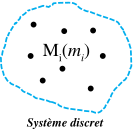
\includegraphics[scale=1]{discret.png}
	\end{center}
	\tcblower
	\tcbsubtitle{\fatbox{\textbf{Système continu}}}
	Un ensemble d'éléments de volumes $\dd{V}$ de masse $\dd{m}$, de position
	$\Mr$.
	\begin{center}
		
\includegraphics[scale=1]{cont.png}
	\end{center}
\end{tcb*}

Sauf cas particuliers, on considèrera des systèmes \textbf{discrets} et
\ul{fermés} (tous les points restent dans le système).

\subsection{Centre d'inertie}
\begin{tcb*}(rapp){Centre d'inertie}
	Le \textbf{centre d'inertie} ou \textbf{centre de gravité} G d'un ensemble
	de points matériels M$_i$ de masses $m_i$ telles que $m\ind{tot} = \sum_i
		m_i$ est défini par~:
	\[
		\boxed{m\ind{tot}\vvr{OG} = \sum_i m_i \vv{{\OMr}_i}}
		\Lra
		\boxed{\sum_i m_i\vv{{\rm GM}_i} = \of}
	\]
	Il s'agit du barycentre des points du système, pondéré par leur masse.
\end{tcb*}

\subsection{Mouvements d'un solide indéformable}

\begin{tcb*}(defi){Solide indéformable}
	Un solide $\Sc$ \textbf{indéformable} est un ensemble de points tels que la
	distance entre deux points quelconques soit constante~:
	\psw{
		\[
			\forall (\Mr_1,\Mr_2) \in ({\rm solide}), \quad {\rm M_1M_2} = \cte
		\]
	}
	\vspace{-15pt}
\end{tcb*}
\begin{tcb*}(impl)<lftt>{Solide indéformable et repère}
	Du fait de ce caractère indéformable, on peut donc associer à un solide
	\textbf{un repère qui lui est propre}. Il suffit de prendre une origine
	quelconque dans le solide et trois axes pointant vers d’autres points du
	solide.
\end{tcb*}
\begin{tcb*}(exem)<lftt>{Solides déformables ou non}
	\begin{isd}[sidebyside align=top]
		\begin{itemize}
			\item Une toupie est un solide~:
		\end{itemize}
		\begin{center}
			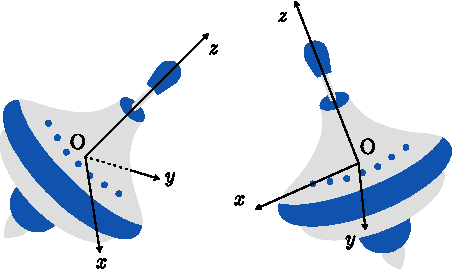
\includegraphics[width=\linewidth]{toup_indef}
		\end{center}
		\tcblower
		\begin{itemize}
			\item Une corde détendue n'est pas un solide~:
		\end{itemize}
		\begin{center}
			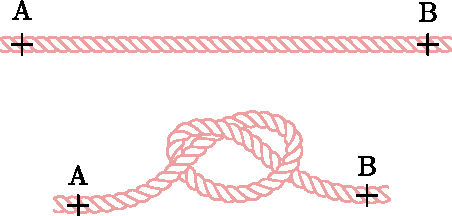
\includegraphics[width=\linewidth]{cord_def}
		\end{center}
	\end{isd}
\end{tcb*}

Un solide peut avoir un mouvement complexe. Dans le cadre du programme, on se
limite à deux situations.

\subsubsection{Translation}
\begin{tcb*}[sidebyside](defi){Mouvement de translation}
	Un solide $\Sc$ en mouvement est en \textbf{translation} si son
	\textbf{orientation est fixe} au cours du mouvement. Ainsi, de manière
	équivalente~:
	\begin{enumerate}
		\item $\forall (\Mr_1,\Mr_2) \in \Sc, \quad
			      \psw{\vvr{M_1M_2} = \vcte}$~;
		\item $\forall t, \forall (\Mr_1,\Mr_2) \in \Sc, \quad
			      \psw{\vf(\Mr_1) = \vf(\Mr_2)}$.
	\end{enumerate}
	\tcblower
	Alors, la connaissance du mouvement \textbf{d'un point} du solide en
	translation permet de connaître le mouvement de \textbf{tout point} du
	solide~; on prendra habituellement le \textbf{centre d'inertie}.
\end{tcb*}

\begin{tcb*}[breakable](exem)<lftt>'l'{Mouvements de translation}
	\begin{enumerate}
		\item \textbf{Translation quelconque}~:
		      \begin{center}
			      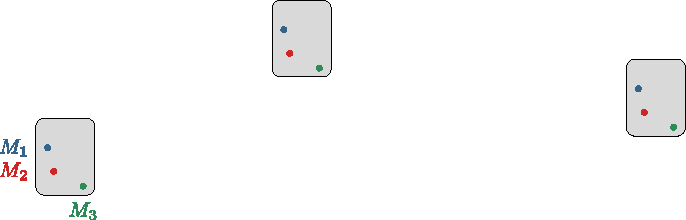
\includegraphics[scale=1]{trans_qlcq}
		      \end{center}
		\item \textbf{Translation rectiligne}~: chaque point décrit une droite.
		      \begin{center}
			      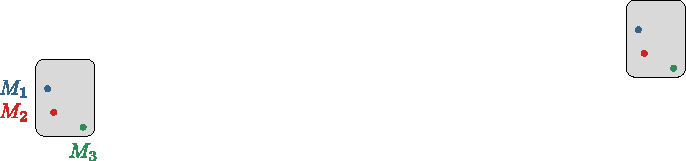
\includegraphics[scale=1]{trans_rect}
		      \end{center}
		      \newpage
		\item \textbf{Translation circulaire}~: chaque point décrit un arc de
		      cercle.
		      \begin{center}
			      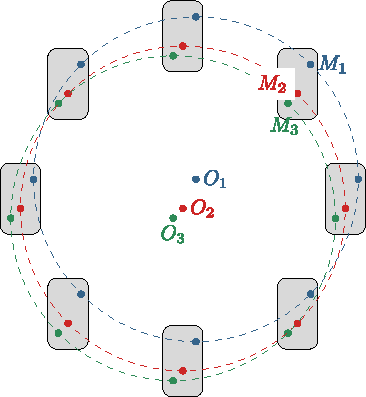
\includegraphics[scale=1]{trans_circ}
		      \end{center}
	\end{enumerate}
\end{tcb*}

\subsubsection{Rotation}
\begin{tcb*}[sidebyside, righthand ratio=.4](defi){Mouvement de rotation et vecteur rotation}
	Un solide est dit en \textbf{mouvement de rotation} autour d'un \textbf{axe
		fixe} $\D$ si la distance de tout point du solide à tout point de l'axe est constante~:
	\psw{
		\[
			\forall \Mr \in \Sc, \forall A \in \Delta, \quad \norm{\vvr{AM}} = \cte
		\]
	}
	Alors, tous les points ont un \textbf{mouvement circulaire} autour de cet
	axe, avec la \textbf{même vitesse angulaire} $\w(t) = \tp(t)$.
	\smallbreak
	On introduit alors le \textbf{vecteur rotation} $\wf$\ftn{parfois noté $\Wf$}
	en $\si{rad.s^{-1}}$ tel que
	\psw{
		\[
			\boxed{\wf_{\Sc/\Rc} = \w(t)\vv{u_\D}}
		\]
	}
	\vspace{-15pt}
	\tcblower
	\begin{center}
		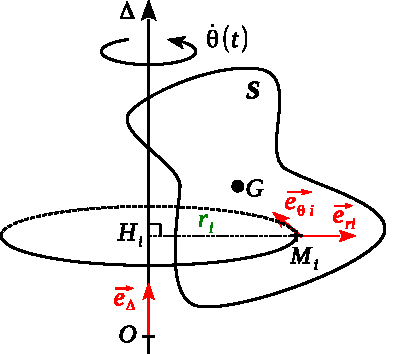
\includegraphics[width=.8\linewidth]{sol_rot}
		\captionof{figure}{Solide en rotation.}
	\end{center}
\end{tcb*}
\begin{tcbraster}[raster equal height=rows, raster columns=2]
	\begin{tcb*}(prop){$\protect\vv{v}_{\Mr}$ pour $\Sc_{rot}$}
		En plaçant un point O sur l'axe de rotation $\Delta$, la vitesse d'un point
		M du solide est
		\psw{
			\[
				\boxed{\vf_{\Mr/\Rc}(t) = \vv{\W}_{\Sc/\Rc} \wedge \OM}
			\]
		}
		\vspace{-15pt}
	\end{tcb*}
	\begin{tcb*}(demo)<rgtt>'r'{$\protect\vv{v}_{\Mr}$ pour $\Sc_{rot}$}
		\vspace{-15pt}
		\psw{
			\begin{align*}
				\OM                          & = r_{\Mr}\ur + z\ud
				\\\Ra
				\wf_{\Sr} \wedge \OM         & =
				\w(t)\ud \wedge \left( r_{\Mr}\ur + \cancel{z\ud} \right)
				\\\Lra
				\Aboxed{\wf_{\Sr} \wedge \OM & = r_{\Mr}\w(t) \ut}
				\qed
			\end{align*}
		}
		\vspace{-15pt}
	\end{tcb*}
\end{tcbraster}

\begin{tcb*}(rema)<lftt>{Vitesse des points d'un solide en rotation}
	\begin{itemize}
		\item On retrouve que la vitesse est nulle sur un point de l'axe,
		      puisqu'alors $\OM \parr \Delta$ donc le produit vectoriel est nul~;
		\item On retrouve que le déplacement des points se fait perpendiculairement
		      à l'axe de rotation (par construction-même du produit vectoriel)~;
		\item Plus on s'éloigne de l'axe, plus la vitesse des points est élevée.
	\end{itemize}
\end{tcb*}

\begin{tcb*}(exem)<lftt>'l'{Mouvements de rotation}
	\begin{isd}
		\begin{center}
			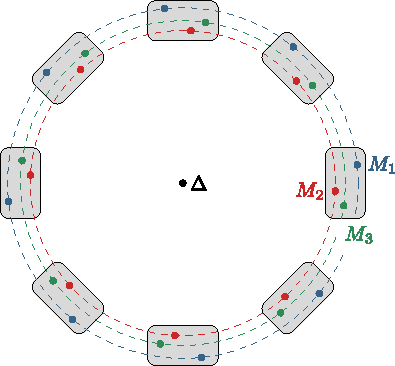
\includegraphics[width=\linewidth]{rot_D}
			\captionof{figure}{Rotation autour de l'axe $\D$ fixe}
		\end{center}
		\tcblower
		\begin{center}
			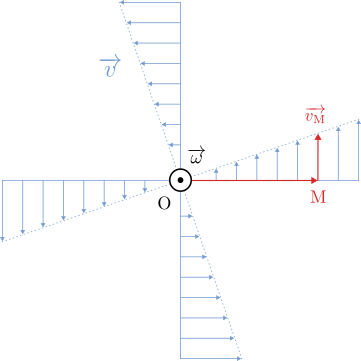
\includegraphics[width=\linewidth]{rot_dist.png}
			\captionof{figure}{Augmentation de la vitesse avec le rayon.}
		\end{center}
	\end{isd}
\end{tcb*}

\begin{tcb*}[tabularx={l|Y|Y|Y}](impo){Ne pas confondre translation circlaire et rotation}
	&
	\textbf{Translation circulaire} & \textbf{Rotation autour d'un axe fixe}
	\\\hline
	\rotatebox[origin=c]{90}{Définition} &
	Tous les points suivent une trajectoire circulaire de même rayon mais de
	centre différent                & Tous les points suivent une trajectoire circulaire de
	même centre mais de rayon différent.
	\\\hline
	\rotatebox[origin=c]{90}{Schéma} &
	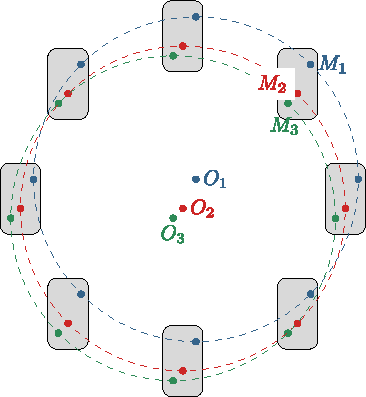
\includegraphics[width=5cm]{trans_circ}
	&
	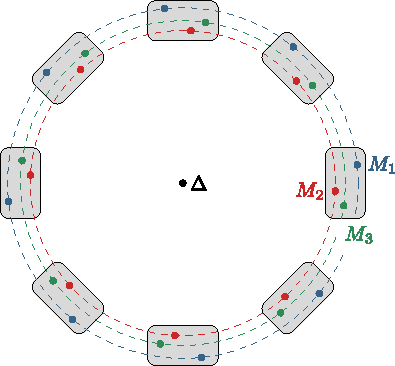
\includegraphics[width=5cm]{rot_D}
	\\[1em]\hline
	\rotatebox[origin=c]{90}{Photo} &
	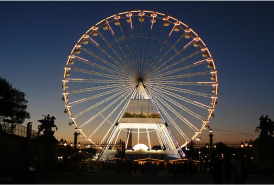
\includegraphics[height=5cm]{trans_roue}
	&
	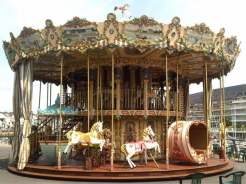
\includegraphics[height=5cm]{rot_carr}
	\\
\end{tcb*}


\subsubsection{Combinaison des mouvements}
\begin{tcb*}(prop){Vitesse des points d'un solide (HP)}
	Lors d'un mouvement plus complexe combinant translation et rotation, la
	vitesse d'un point M du solide est donnée par~:
	\psw{
		\[
			\boxed{\vf_{\Mr/\Rc} = \vf_{\Or} + \vv{\W}\wedge \OM}
		\]
	}
	\vspace{-15pt}
\end{tcb*}

\section{Rappel~: TRC}
\subsection{Quantité de mouvement d'un ensemble de points}

On souhaiterait pouvoir étudier un ensemble de points comme le mouvement d'un
point unique, comme le centre d'inertie. Pour cela, il faut étudier la quantité
de mouvement d'un ensemble de points.

\begin{tcb*}(defi){Quantité de mouvement d'un ensemble de points}
	Le vecteur quantité de mouvement d'un ensemble $\Sc$ de points matériels
	M$_i$ de masses $m_i$ est défini par~:
	\psw{\[\boxed{\pf(\Sc) = \sum_i\pf(\Mr_i) = \sum_i m_i \vf(\Mr_i)}\]}
\end{tcb*}

% Pour que les choses soient simples, il faudrait donc que $\pf(\Sc)$ soit relié
% au centre d'inertie. Ça tombe bien~:

\begin{tcb*}[cnt, bld](prop){Quantité de mouvement d'un système}
	La quantité de mouvement d'un ensemble de points est la quantité de
	mouvement d'un point matériel placé en G et de masse $m_{\tot}$~:
	\psw{\[\boxed{\pf(\Sc) = m_{\tot}\vf(\Gr)}\]}
	Tout se passe comme si la masse était concentrée en G.
\end{tcb*}

\begin{tcb*}(demo)<lftt>{$\protect\pf_{\Sc}$}
	\psw{
		\begin{gather*}
			m_{\tot}\vf(\Gr) = m_{\tot}\dv{\vvr{OG}}{t} =
			\underbrace{\sum_i m_i \dv{\vv{\OMr_i}}{t}}_{\pf(\Sc)}
			\Lra
			\boxed{\pf(\Sc) = m_{\tot}\vf(\Gr)}
			\qed
		\end{gather*}
	}
	\vspace{-15pt}
\end{tcb*}

\subsection{Forces intérieures et extérieures}
Si on peut étudier la cinématique d'un corps par l'étude de son centre de
gravité, comment les forces interviennent-elles sur cet ensemble de points~?
Les forces s'appliquant aux points M$_i$ de $\Sc$ se rangent en deux
catégories~:
\begin{enumerate}
	\item Les forces intérieures $\Ff_{\rint\ra\Mr_i}$ exercées par les autres
	      points M$_j$ du système, avec $j\neq i$~;
	\item Les forces extérieures $\Ff_{\ext\ra\Mr_i}$ exercées par une origine
	      externe au système.
\end{enumerate}
Les forces intérieures ont cependant une propriété remarquable~:
\begin{tcb*}[cnt, bld](prop){Résultante des forces intérieures}
	La résultante $\Ff_{\rint}$ des forces intérieures d'un système est toujours
	nulle.
\end{tcb*}
\begin{tcb*}(demo)<lftt>{Résultante des forces intérieures}
	La résultante des forces intérieures exercées sur M$_i$ s'écrit
	\psw{
		\[
			\Ff_{\rint\ra i} = \sum_{j\neq i}\Ff_{j\ra i}
		\]
	}%
	Ainsi la résultante des forces intérieures au système s'écrit
	\psw{
		\[
			\Ff_{\rint} = \sum_i \Ff_{\rint\to i} = \sum_i\sum_{j\neq i}\Ff_{j\to
				i}
		\]
	}%
	Or, d'après la troisième loi de \textsc{Newton}, \psw{$\forall i\neq j, \quad
			\Ff_{j\to i} = -\Ff_{i\to j}$}~; ainsi, les termes de la somme précédente
	s'annulent deux à deux, et on a bien
	\psw{
		\begin{gather*}
			\boxed{\Ff_{\rint} = \sum_i\Ff_{\rint\to i} = \of}
			\qed
		\end{gather*}
	}
	\vspace{-15pt}
\end{tcb*}
Rien de remarquable ne se produit pour les forces extérieures, et on aura
simplement
\[\boxed{\Ff_{\ext} = \sum_i \Ff_{\ext\to i}}\]

\subsection{Théorème de la résultante cinétique}
% Considérons pour simplifier un système de deux points M$_1$ et M$_2$ de masses
% $m_1$ et $m_2$ en mouvement dans un référentiel galiléen. On peut appliquer le
% principe fondamental de la dynamique à chacun d'entre eux~:
% \[\dv{\pf(\Mr_1)}{t} = \Ff_{\Mr_2\ra\Mr_1} + \Ff_{\ext\ra\Mr_1}\]
% avec deux types de forces~: les forces intérieures du système, ici celles
% exercées par M$_2$ sur M$_1$, et les forces extérieures, c'est-à-dire toutes les
% autres. En faisant de même pour M$_2$~:
% \[\dv{\pf(\Mr_2)}{t} = \Ff_{\Mr_1\ra\Mr_2} + \Ff_{\ext\ra\Mr_2}\]
% Ainsi, avec la définition de la quantité de mouvement d'un ensemble de points,

\begin{tcbraster}[raster columns=2, raster equal height=rows, raster
		valign=top]%
	\begin{tcb*}(theo){de la résultante cinétique}
		Le PFD pour un M s'applique à $\Sc$ en prenant pour point matériel le
		\textbf{centre d'inertie} G affecté de la \textbf{masse totale} $m_{\tot}$
		du système, en ne considérant que les \textbf{forces extérieures}
		s'appliquant à l'ensemble~:
		\psw{
			\[
				\boxed{\dv{\pf\Rg(\Sc)}{t} = m_{\tot}\dv{\vf(\Gr)}{t} = \Ff_{\ext}}
			\]
		}
		\vspace{-15pt}
	\end{tcb*}%
	\begin{tcb*}(demo)<lftt>'r'{TRC}
		\psw{
			\begin{align*}
				\dv{\pf\Rg(\Sc)}{t}         & = \sum_i \dv{\pf\Rg(\Mr_i)}{t}
				\\
				                            & = \underbracket[1pt]{
					\sum_i \Ff_{\rint\to i}
				}_{=\of\text{ par 3\ieme\ loi}} +
				\underbracket[1pt]{
					\sum_i \Ff_{\ext\to i}
				}_{=\Ff_{\ext}\text{ par déf.}}
				\\\Lra
				\Aboxed{\dv{\pf\Rg(\Sc)}{t} & = m_{\tot}\dv{\vf(\Gr)}{t} = \Ff_{\ext}}
				\qed
			\end{align*}
		}
	\end{tcb*}
\end{tcbraster}
\begin{tcb*}(impo){Utilisation du TRC}
	Ce théorème ne contient que l'\textbf{information du centre d'inertie}~; il ne
	suffit pas à décrire tout le système, notamment les rotations pures~!
\end{tcb*}

\section{Énergétique des systèmes de points}
On l'a vu dans les chapitres précédents, différentes approches sont possibles en
mécanique selon le résultat désiré. Si le PFD permet d'avoir l'information
dynamique sur le centre d'inertie, on cherche à établir les résultats de
l'approche énergétique aux solides. Commençons par le plus simple~:
\subsection{Cinétique}
\begin{tcb*}(defi){Énergie cinétique d'un système de points}
	Comme pour la masse ou la quantité de mouvement, l'énergie cinétique d'un
	solide est la \textbf{somme des énergies cinétiques de chaque point le
		constituant}~:
	\psw{
	\[
		\boxed{\Ec_{c/\Rc}(\Sc) = \sum_i\Ec_{c/\Rc}(\Mr_i) = \sum_i
		\frac{1}{2}m_iv_{i/\Rc}{}^2}
	\]
	}
	\vspace{-15pt}
\end{tcb*}

\subsection{Puissance intérieure}
Pour pouvoir appliquer les théorèmes énergétiques, il faut détailler les
puissances des forces s'appliquant au solide, et notamment les forces
intérieures. Les points M$_j$ avec $j\neq i$ exercent des forces sur M$_i$. La
puissance de ces actions s'exprime~:
\[\Pc_{\rint\to i} = \sum_{j\neq i} \Ff_{j\to i}\cdot\vf_i\]
Seulement, on a la propriété suivante~:
\begin{tcb*}(prop){Puissance des forces intérieures}
	\begin{center}
		\begin{bfseries}
			La puissance des forces intérieures est nulle \ul{pour un système
				indéformable}.
		\end{bfseries}
	\end{center}
\end{tcb*}
\begin{tcb*}(demo)<lftt>{Puissance des forces intérieures}
	En effet, la puissance de toutes les forces intérieures s'exprime
	\[
		\Pc_{\rint} =
		\sum_i\Pc_{\rint\to i} =
		\sum_i\sum_{j\neq i}\Ff_{j\to i}\cdot \vf_i =
		\sum_i\sum_{j\neq i}\Ff_{j\to i}\cdot \dv{\vv{\Mr_j\Mr_i}}{t}
	\]
	Or, pour un solide en translation, $\Mr_j\Mr_i = \vcte$ par construction. Ça
	pourrait ne pas être le cas pour un solide en rotation, puisque le vecteur
	n'est pas fixe. On peut pour cela étudier précisément deux puissances entre
	M$_i$ et M$_j$~: on a, dans la base sphérique $(\Mr_j, \vv{u}_{r,j\to i},
		\vv{u}_{\th,j\to i}, \vv{u}_{\f,j\to i})$~:
	\begin{gather*}
		\Ff_{j\to i} = F_{j\to i}\vv{u}_{r,j\to i} \qquad \text{force centrale due au
			contact}\\
		\dv{\vv{\Mr_j\Mr_i}}{t} = \rp_{i,j}\vv{u}_{r,j\to i} +
		r_{i,j}\tp_{i,j}\vv{u}_{\th,j\to i} + r_{i,j}\sin\th_{i,j}\vv{u}_{\f,j\to i}
		\\\Lra
		\Ff_{j\to i}\cdot\dv{\vv{\Mr_j\Mr_i}}{t} = F_{j\to i}
		\underbracket[1pt]{\rp_{i,j}}_{\mathclap{=0~\text{car indéformable}}}
		\\\Lra
		\boxed{\Pc_{\rint} = 0}
		\qed
	\end{gather*}
\end{tcb*}

\subsection{Théorèmes}
On retrouve ainsi les théorèmes utilisés pour le point, en prenant alors en
compte les forces intérieures~:
\begin{tcb*}(theo){Énergétique pour le solide}
	Pour un système $\Sc$ dans un référentiel galiléen $\Rc$~: \smallbreak
	\begin{isd}
		\begin{center}
			\tcbsubtitle{\fatbox{\textbf{TEC, TPC}}}
		\end{center}
		\begin{empheq}[box=\fbox]{align*}
			\D\Ec_{c/\Rc} &= W_{\ext/\Rc} + W_{\rint/\Rc}\\
			\dv{\Ec_{c/\Rc}}{t} &= \Pc_{\ext/\Rc} + \Pc_{\rint/\Rc}
		\end{empheq}
		\tcblower
		\begin{center}
			\tcbsubtitle{\fatbox{\textbf{TEM, TPM}}}
		\end{center}
		\begin{empheq}[box=\fbox]{align*}
			\D\Ec_{m/\Rc} &= W_{\ext,NC/\Rc} + W_{\rint, NC/\Rc}\\
			\dv{\Ec_{m/\Rc}}{t} &= \Pc_{\ext,NC/\Rc} + \Pc_{\rint,NC/\Rc}
		\end{empheq}
	\end{isd}
\end{tcb*}

\begin{tcb*}(demo)<lftt>{Énergétique pour le solide}
	Il suffit d'appliquer le TPC ou TPM à chaque point matériel M$_i$ du
	système.
\end{tcb*}

\section{Moments pour un système de points}
\subsection{Moment cinétique et moment d'inertie}
Comme pour le reste des grandeurs, le moment cinétique d'un système de points
est la somme des moments cinétiques de chaque point~:
\begin{tcb*}(defi){Moment cinétique d'un système}
	Par rapport à un point O fixe dans $\Rc$ référentiel d'étude~:
	\[
		\boxed{\Lcf_{\Or/\Rc}(\Sc) = \sum_i\Lcf_{\Or/\Rc}(\Mr_i)
			= \sum_i \OM_i\wedge\pf\Rg(\Mr_i)}
	\]
\end{tcb*}
\begin{tcb*}(prop){Moment cinétique et moment d'inertie d'un solide}
	Le moment cinétique d'un solide en rotation est proportionnel à la vitesse
	angulaire $\wf = \w(t)\ud$~:
	\[
		\boxed{
			\Lcf_{\Or} = J_{\D}\wf
			\Lra
			\Lc_z = J_{\D}\w
		}
	\]
	avec $J_{\D}$ le moment d'inertie.
\end{tcb*}
\begin{tcb*}(demo){Moment d'inertie d'un solide}
	Pour un solide en rotation autour de l'axe $z$, on aura
	\smallbreak
	\begin{isd}[sidebyside align=top]
		\tcbsubtitle{\fatbox{\textbf{Discret}}}
		\begin{align*}
			\Lc_z(\Mr_i) & = (\OM_i\wedge m_i\vf_i)\cdot\uz
			\\\Lra
			\Lc_z(\Mr_i) & = (r_i\ur)\wedge(m_ir_i\tp_i\ut)\cdot\uz
			\\\Lra
			\Lc_z(\Mr_i) & = m_ir_i{}^2\tp_i\,
			\underbracket[1pt]{\ur\wedge\ut}_{=\uz}\cdot\uz = m_ir_i{}^2\tp_i
			\\
			\beforetext{Or}
			\Lc_z(\Sc)   & = \sum_i \Lc_z(\Mr_i)
			\\\Lra
			\Lc_z(\Sc)   & = \sum_i m_ir_i{}^2\tp_i
			\qed
		\end{align*}
		\tcblower
		\tcbsubtitle{\fatbox{\textbf{Continu (HP)}}}
		\begin{gather*}
			J_z = \int \dm\,r^2
		\end{gather*}
	\end{isd}
\end{tcb*}

\begin{tcb*}(inte)<lftt>{Correspondance quantité de mouvement et quantité de rotation}
	Le moment d'inertie caractérise \textbf{l'inertie de rotation}, c'est-à-dire
	la facilité avec laquelle la rotation d'un solide s'établit ou s'arrête~; il
	est analogue à la \textbf{masse} pour la translation, qui caractérise
	l'inertie d'un corps à être mis en mouvement. On peut en effet associer
	\[
		\pf = m\vf
		\qqet
		\Lcf_{\Or} = m\wf
	\]
	et tous les théorèmes en découlant par ailleurs.
\end{tcb*}

\begin{tcb*}[cnt, bld](ror){Analyse du moment d'inertie}
	Plus la masse d'un solide est excentrée, plus le moment d'inertie
	est grand et plus il est difficile de le mettre en rotation.
\end{tcb*}

\begin{tcb*}(exem)<lftt>'l'{Moments d'inertie divers}
	\begin{itemize}
		\item Point matériel distance $R$, $J_z = mR^2$~;
		\item Barre en rotation centrale~: $J_z = \frac{mL^2}{12}$~;
		\item Barre en rotation à son extrémité~: $J_z = \frac{mL^2}{3}$~;
		\item Boule pleine en rotation axiale~: $J_z = \frac{2}{5}mR^2$.
	\end{itemize}
\end{tcb*}
\subsection{Moments intérieurs}
Olivier

\subsection{TMC}
Olivier

Analogie Schweitzer

\subsection{Énergie cinétique de rotation}
Schweitzer

\section{Cas particuliers et application}
Schweitzer~: couple, pivot~; aucun moment = pas de frottements

Schweitzer pendule pesant

\end{document}
